% =====================================================================
%  APPENDIX --- Phase-1 Apollo HFE validation (book-like SI)
%
%  This document accompanies "Single-Pixel Validation of the
%  Diviner-Derived Global Lunar Regolith Thermophysical Model at the
%  Apollo 15 and 17 Heat-Flow Experiment Sites" (the Letter).
%  It is intentionally written for a reader with little or no prior
%  background in lunar regolith physics, numerical heat transfer, or
%  the SPICE toolkit. Anyone who has taken one undergraduate PDE
%  course should be able to read it cover-to-cover.
% =====================================================================
\documentclass[11pt]{report}

\usepackage[a4paper,margin=2.4cm]{geometry}
\usepackage[T1]{fontenc}
\usepackage{lmodern}
\usepackage{microtype}
\usepackage{amsmath,amssymb,amsthm}
\usepackage{siunitx}
\sisetup{detect-all,per-mode=symbol}
\usepackage{graphicx}
\usepackage{booktabs}
\usepackage{caption,subcaption}
\captionsetup{font=small,labelfont=bf,labelsep=period}
\usepackage[hidelinks,colorlinks=true,linkcolor=blue!50!black,
            citecolor=blue!50!black,urlcolor=blue!60!black]{hyperref}
\usepackage{xcolor}
\usepackage{tcolorbox}
\tcbuselibrary{skins,breakable}
\usepackage[round,authoryear]{natbib}
\bibliographystyle{plainnat}
\usepackage{listings}
\lstset{
  basicstyle=\ttfamily\footnotesize,
  numbers=left, numberstyle=\tiny\color{gray!70},
  frame=single, framesep=4pt, rulecolor=\color{gray!40},
  backgroundcolor=\color{gray!5},
  language=Python, keywordstyle=\color{blue!50!black}\bfseries,
  commentstyle=\color{green!40!black}\itshape,
  stringstyle=\color{red!50!black},
  breaklines=true, showstringspaces=false,
  captionpos=b, xleftmargin=12pt
}

% Coloured boxes for pedagogical asides
\newtcolorbox{aside}[1][Aside]{enhanced,colback=blue!4,colframe=blue!40!black,
  fonttitle=\bfseries,title={#1},breakable}
\newtcolorbox{warn}[1][Pitfall]{enhanced,colback=red!4,colframe=red!50!black,
  fonttitle=\bfseries,title={#1},breakable}
\newtcolorbox{key}[1][Key result]{enhanced,colback=green!4,colframe=green!40!black,
  fonttitle=\bfseries,title={#1},breakable}

% --- Convenience macros --------------------------------------------------
\newcommand{\Hayne}{Hayne (\citeyear{hayne2017})}
\newcommand{\Vas}{Vasavada \emph{et~al.} (\citeyear{vasavada2012})}
\newcommand{\dT}{\Delta T}
\newcommand{\zborestem}{80\,\si{\centi\meter}}

\title{\bfseries Supporting Information for\\
``Regional Heterogeneity in Lunar Deep Regolith Conductivity\\
from a Per-Site Retrieval Against the Restored Apollo 15 and 17\\
Heat-Flow Experiment Record''\\[6pt]
\large A Self-Contained Walk-Through of the Methodology}
\author{R.~P.~Gregorio}
\date{\today}

\begin{document}
\maketitle
\tableofcontents
\clearpage

% =====================================================================
\chapter*{How to read this document}\addcontentsline{toc}{chapter}{How to read this document}

This Supporting Information (SI) is written as a self-contained tutorial.
Each chapter starts from first principles and assumes only an undergraduate
background in differential equations, basic statistics, and rudimentary
Python. If you are an experienced lunar thermophysics modeller, you may
skim Chapters~\ref{ch:moon}--\ref{ch:numerics} and jump to
Chapter~\ref{ch:validation}. If you are a planetary-science student or
non-specialist reader opening these methods for the first time, please
start with Chapter~\ref{ch:plain} (a non-technical narrative of the
entire study) before reading the rest in order.

\medskip\noindent\textbf{Visual conventions} (used throughout):

\begin{aside}[Aside]
Coloured \emph{aside} boxes contain pedagogical context, intuition, or
historical notes that the main text does not strictly require but which
help build understanding.
\end{aside}

\begin{key}[Key result]
Green \emph{key result} boxes contain a takeaway you should remember
after reading the surrounding section.
\end{key}

\begin{warn}[Pitfall]
Red \emph{pitfall} boxes flag a place where it is easy to make a
subtle mistake; we describe the mistake and the way to avoid it.
\end{warn}

% =====================================================================
\chapter{What this study did, in plain English}\label{ch:plain}

This chapter is for the reader who wants to understand what was
done, why it matters, and how each piece fits together --- without
having to follow any equations. Every technical concept introduced
here is unpacked in a later chapter, and a forward-pointer
(``\textsection{}~XX.X'') tells you where to look. If something here
is unclear, the right move is to read this chapter once for the
narrative and then dip into the later chapters as the equations
become relevant.

% ---------------------------------------------------------------------
\section{The setting}

The Moon has no atmosphere and no oceans, so its surface heats and
cools by hundreds of kelvin every $\sim$29.5-Earth-day lunar day.
The thin, broken-up layer of rock at the surface --- the
\emph{regolith} --- is what insulates the deeper interior from those
extreme swings. How effectively it insulates is determined mostly
by a single material property, the \emph{thermal conductivity} (the
ability to carry heat through the material). Most spacecraft analyses
of the Moon, including calculations of how stable buried water-ice is
near the poles and how hot a future lander's payload will get, treat
this conductivity as a single fixed number that applies everywhere on
the Moon. That assumption has never been tested directly, because
nobody has ever measured the conductivity of the deep regolith
\emph{in place} --- only inferred it from how the surface looks in
infrared images from orbit.

% ---------------------------------------------------------------------
\section{The data we used}

In 1971 and 1972, the Apollo~15 and Apollo~17 astronauts buried two
arrays of thermometers $\sim$2.4--2.5 metres deep into the lunar
surface. These thermometers ran almost continuously until 1977 and
recorded the only \emph{in-situ} measurements of subsurface
temperature ever made on the Moon. The original data tapes were lost
for decades. \citet{nagihara2018} restored the full
1971--1977 record, and that restored record is the dataset we use
here. The detailed instrument description is in \S\ref{ch:moon}.

% ---------------------------------------------------------------------
\section{The model we built}

We built a one-dimensional, time-dependent computer model of the
heat flow through a vertical column of regolith. At each instant
the model takes the sunlight falling on the surface (computed from
exact spacecraft-grade ephemerides; \S\ref{ch:hayne}) and asks: given
the regolith's thermal properties, what temperature does each depth
settle to over many lunar days? Solving that question requires a
numerical scheme called Crank--Nicolson (\S\ref{ch:numerics}); think
of it as a careful bookkeeping algorithm that updates every depth in
the column by a small time step, conserves energy at each step, and
is stable enough to keep running for hundreds of simulated lunar days
without drifting.

The thermal properties --- conductivity, density, and heat capacity
--- come from a published global model by \citet{hayne2017} that was
fit to infrared brightness measurements taken from orbit. We use
their model exactly as published, except that we treat one number
(the deep conductivity, called $K_d$) as adjustable rather than
fixed.

% ---------------------------------------------------------------------
\section{The single experiment}

The experiment is a one-parameter fit. We sweep the deep
conductivity $K_d$ across a range of plausible values, run the full
heat-flow model for each value, and ask: which $K_d$ makes the
model's predicted deep temperatures best match the Apollo
thermometer readings? We do this independently for each landing
site. The full procedure is in \S\ref{ch:validation}.

There is one subtlety. The shallow thermometers (above
$\sim$80~cm depth) are known to be contaminated: they are mounted
inside fibreglass tubes that conduct heat down from the
\emph{surface}, where the temperature swings are huge, and so they
read warmer than the regolith would predict on its own. We exclude
those shallow readings from our fit. Crucially, we identify which
sensors to exclude using a \emph{model prediction} --- specifically,
the predicted day--night swing as a function of depth --- rather than
by looking at where our model fits the data poorly. This avoids the
trap of throwing away exactly the data points the model fails on.

% ---------------------------------------------------------------------
\section{What we found}

When we run the experiment, the two Apollo sites give very different
answers:

\begin{itemize}\itemsep2pt
  \item Apollo~15 prefers $K_d \approx 4.85$~mW/(m\,K).
  \item Apollo~17 prefers $K_d \approx 11.23$~mW/(m\,K).
\end{itemize}

The published global value is 3.4~mW/(m\,K). Both sites
\emph{disagree} with the published value, and the two sites disagree
\emph{with each other} by more than a factor of two. The disagreement
is much larger than the uncertainty on either measurement
(quantitatively, $\sim$7.5 standard deviations on a leave-one-out
jackknife; \S\ref{ch:validation}).

% ---------------------------------------------------------------------
\section{Why that matters}

Two things follow from this result.

\textbf{First}, the thermal conductivity of the deep lunar regolith
is regionally heterogeneous --- it is genuinely different at
different places on the Moon, even at non-polar latitudes where the
regolith is comparatively well-studied. Whether this reflects
differences in mineralogy, in compaction with depth, in particle-size
distribution, or in some other property that varies regionally, is a
question for follow-up work. But the assumption that one global value
of $K_d$ describes the whole Moon is not consistent with the in-situ
data.

\textbf{Second}, anyone using the published global value to compute
the cold-trap depth where polar water-ice is stable, or to set the
heat budget for a lander instrument, is implicitly accepting an
uncertainty at least as large as the inter-site disagreement we
report. That uncertainty is large enough to matter for several
mission-design questions, and it should be reflected in the error
bars of any analysis that propagates $K_d$ through a temperature
calculation.

% ---------------------------------------------------------------------
\section{What this study cannot tell you}

There is one important caveat. The two unknowns at the bottom of any
buried-thermometer column are the deep conductivity $K_d$ and the
heat coming up from the deep interior, $Q_b$. At long times the
two unknowns enter the equilibrium temperature gradient
\emph{only as their ratio} $Q_b/K_d$, so any single buried column
cannot tell them apart on its own. We adopt the canonical published
$Q_b$ values for each site (\citealt{langseth1976,nagihara2018}), and
the absolute $K_d$ we report inherits whatever uncertainty those
values carry --- about $\pm$30\% at A15.

The good news is that the \emph{difference} between A15 and A17 is
not affected by this caveat: any global rescaling of $Q_b$ rescales
both sites equally, leaving the contrast fixed. So the central
finding (regional heterogeneity) is robust to the $Q_b$ uncertainty;
the absolute A17 number is not. We discuss this in detail in
\S\ref{ch:validation}.

% ---------------------------------------------------------------------
\section{Where to read next}

The rest of this document fills in each piece of the narrative
above:

\begin{itemize}\itemsep2pt
  \item Chapter~\ref{ch:moon} --- the lunar thermal environment
        and how the Apollo HFE instrument actually worked.
  \item Chapter~\ref{ch:pde} --- the heat equation, derived from
        first principles.
  \item Chapter~\ref{ch:hayne} --- the \citet{hayne2017} regolith
        property functions, and the SPICE/DE440 surface-forcing
        chain that drives the model.
  \item Chapter~\ref{ch:numerics} --- the Crank--Nicolson numerical
        solver and its convergence diagnostics.
  \item Chapter~\ref{ch:validation} --- the per-site $K_d$
        retrieval, including the leave-one-out jackknife
        uncertainty, the borestem-exclusion diagnostic, and the
        $K_d/Q_b$ degeneracy.
  \item Chapter~\ref{ch:crosschecks} --- independent cross-checks
        of the solver.
  \item Chapter~\ref{ch:repro} --- a reproducibility guide that
        walks through the source code file by file.
  \item Chapter~\ref{ch:glossary} --- a glossary of terms and
        symbols.
\end{itemize}

\begin{key}[Take-away]
The study uses Apollo-era buried thermometers to measure the
\emph{insulation strength} of the deep lunar regolith independently
at two landing sites; the two sites disagree by more than a factor of
two; therefore the regolith is regionally heterogeneous, and the
single global value used in current spacecraft analyses understates
the true uncertainty.
\end{key}

% =====================================================================
\chapter{The Moon as a Thermal System}\label{ch:moon}

\section{Why the Moon's surface temperature varies so much}

The Moon has no atmosphere and no oceans. The only things buffering
its surface temperature against the day--night solar cycle are the
\emph{thermal inertia} of the regolith (the loose, broken-up rock
covering the surface) and, to a lesser extent, radiative re-emission
to space. Thermal inertia is conventionally defined as
\begin{equation}
I = \sqrt{K \rho c_p},\qquad
[\,\mathrm{J\,m^{-2}\,K^{-1}\,s^{-1/2}}\,],
\label{eq:inertia}
\end{equation}
where $K$ is thermal conductivity, $\rho$ is bulk density and $c_p$
is specific heat. For the Moon's regolith, $I$ is in the range
$30$--$70$~$\mathrm{J\,m^{-2}\,K^{-1}\,s^{-1/2}}$
\citep{vasavada2012}, hundreds of times \emph{lower} than that of bare
rock and roughly a thousand times lower than ocean water. The
practical consequence is that the lunar surface heats and cools by
several hundred kelvin in a single lunation
\citep[$\sim$\SI{29.53}{\day};][]{paige2010}.

\begin{aside}[Why is regolith such a good insulator?]
The regolith grains are roughly $50\text{--}100\,\mu$m in diameter and
the contacts between them are essentially point contacts. Heat conducts
across point contacts very poorly --- much more poorly than across the
bulk silicate it would be in solid form --- so the effective
$K$ is two to three orders of magnitude below the mineral value.
The radiative term $\chi(T/350)^3$ in (\ref{eq:K-rep}) reflects the
fact that, at high temperature, photons can hop from grain to grain
across the empty pore space, providing a parallel heat-transfer
channel that becomes important above $\sim$200\,\si{\kelvin}.
\end{aside}

\section{The thermal skin depth}

The depth $\delta$ over which a periodic surface temperature wave of
angular frequency $\omega$ attenuates by a factor $e^{-1}$ is the
\emph{skin depth} of that wave:
\begin{equation}
\delta = \sqrt{\frac{2\,\kappa}{\omega}},\qquad
\kappa \equiv \frac{K}{\rho\,c_p},
\label{eq:skin}
\end{equation}
where $\kappa$ is the thermal diffusivity. For the Moon's diurnal
cycle ($\omega = 2\pi/\SI{29.53}{\day}\approx 2.5\times10^{-6}\,\si{\per\second}$)
and a representative $\kappa\approx 10^{-8}\,\si{\meter\squared\per\second}$
near the surface, this gives $\delta\approx \SI{0.06}{\meter}$ ---
exactly the H-parameter (\Hayne) used throughout this work.

\begin{key}[Why we need to model 5\,m of regolith]
The annual skin depth scales as $\delta \propto 1/\sqrt{\omega}$, so the
annual wave penetrates $\sqrt{29.53\times 12}\approx 19$ times deeper than the
diurnal wave: roughly $\SI{1.1}{\meter}$. To capture the deep Apollo
HFE sensors at \SI{2.3}{\meter} \emph{and} the asymptotic geothermal
gradient (which requires a quiet zone several skin depths below the
deepest measurement) we extend the modelled column to $\SI{5}{\meter}$.
\end{key}

Fig.~\ref{fig:skindepth} illustrates this graphically. The left panel
shows synthetic temperature time-series at several depths, all driven
by the same surface diurnal forcing of $\sim\!100$\,K amplitude; the
right panel shows the attenuation factor versus depth. Below
$\zborestem$ the diurnal amplitude has been reduced by 18 e-foldings
to $\sim\!10^{-9}$\,K, explaining why the deep-sensor amplitudes
carry no information about the in-situ regolith thermal diffusivity.

\begin{figure}[hbt]
\centering
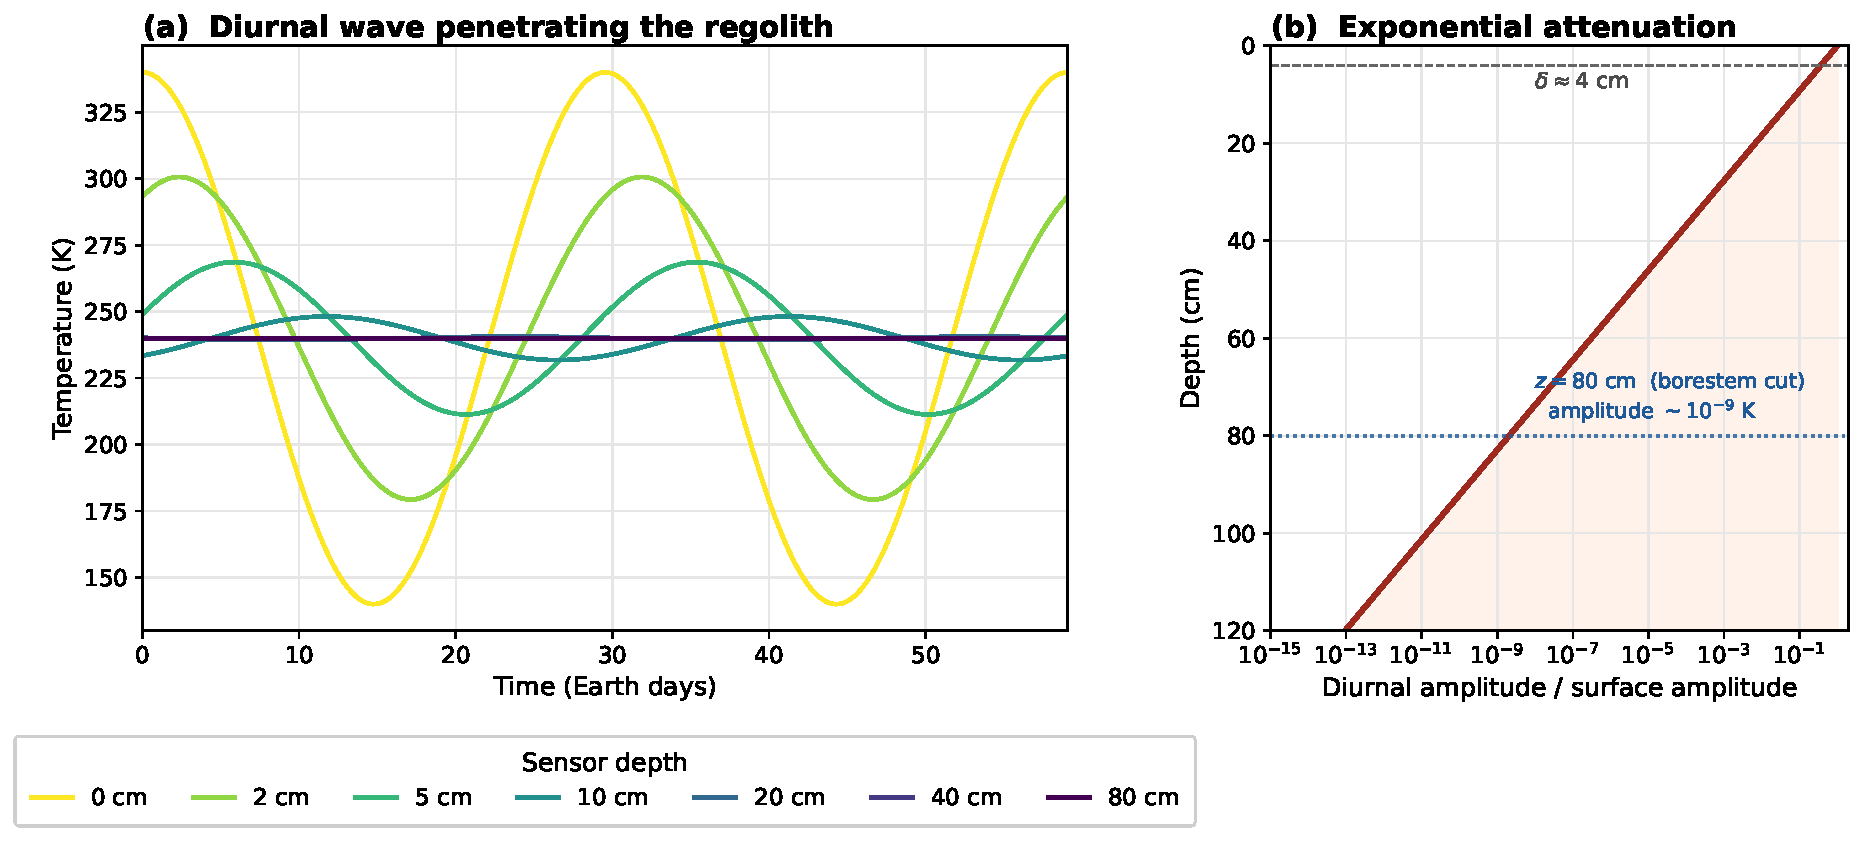
\includegraphics[width=0.99\linewidth]{figures/fig_skin_depth.pdf}
\caption{\textbf{Diurnal-wave attenuation in the lunar regolith.}
(a)~Two lunations of synthetic surface-driven temperature at
selected depths; the surface (yellow) sees the full $\sim\!200$\,K
peak-to-peak diurnal swing while sensors at $40$\,cm and below show
an essentially flat trace. (b)~The corresponding amplitude
attenuation factor $\exp(-z/\delta)$ on a logarithmic axis, with the
e-folding skin depth $\delta\approx 4$\,cm and the borestem-cut
threshold $\zborestem$ marked. Below $\zborestem$ the residual
diurnal amplitude $\sim\!10^{-9}$\,K is many orders of magnitude
below the digitisation noise floor of the restored 1971--1977 record
($\sim\!0.05$--$\SI{0.2}{\kelvin}$).}
\label{fig:skindepth}
\end{figure}

\section{What the Apollo Heat-Flow Experiment actually measured}

Each Apollo~15 and Apollo~17 borehole was drilled to roughly
$\SI{2.4}{\meter}$ (A15) and \SI{2.5}{\meter} (A17) using a hollow
fibreglass tube ("borestem") that was left in place after drilling
to keep the hole open. Inside this tube, a probe carrying eight
platinum-resistance thermometers was lowered to instrumented depths.
Two thermometer types were deployed:

\begin{itemize}\itemsep2pt
  \item \textbf{Gradient (TG) bridges} measured the absolute
        temperature difference between two sensors separated by
        $\sim\SI{50}{\centi\meter}$ along the tube --- designed to
        return the equilibrium thermal gradient and hence (after
        applying a $K$ value) the basal heat flux.
  \item \textbf{Ring (TR) bridges} measured the absolute temperature
        of a single sensor relative to a reference resistor in the
        Apollo Lunar Surface Experiments Package (ALSEP) housing on
        the surface --- designed primarily to track diurnal and
        annual variability.
\end{itemize}

The complete dataset, restored from the original tapes by
\citet{nagihara2018}, covers $\sim\!1971\text{--}1977$ for both sites
and provides the only \emph{in-situ} subsurface temperature
measurements ever made on the Moon.

Fig.~\ref{fig:instrument} shows the geometry of a single Apollo HFE
borehole. The fibreglass borestem extends from the surface down to
the bottom of the hole, and the temperature probe sits inside it.
Sensors above $\zborestem$ are shaded red because they are
contaminated by heat conducted down the borestem from the surface
(see the box below); sensors below $\zborestem$ are shaded blue
because they sit deep enough that the borestem heat-short is
negligible relative to the regolith conductive flux.

\begin{figure}[hbt]
\centering
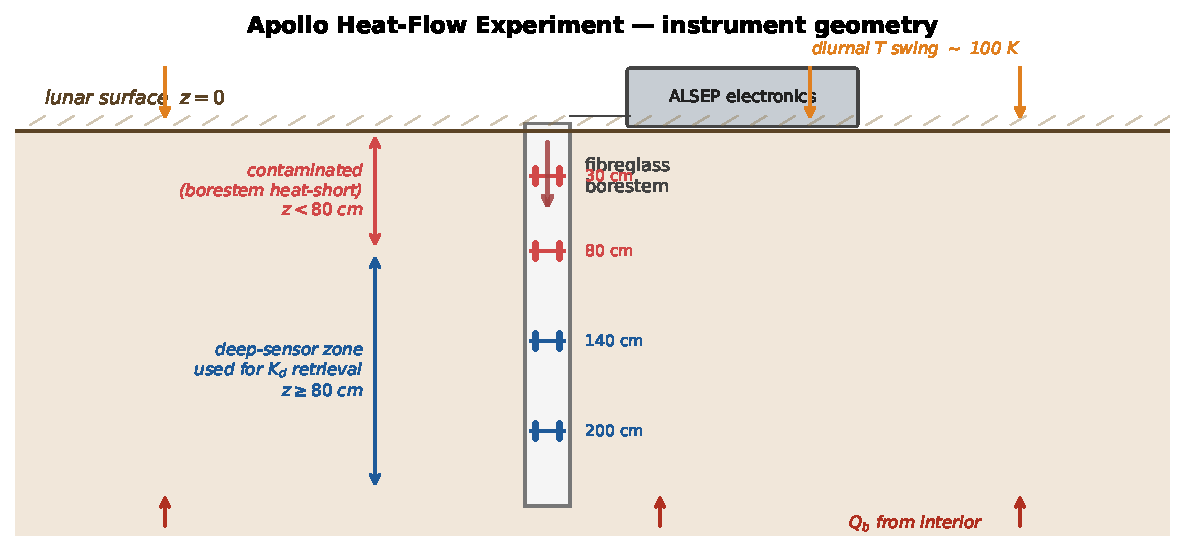
\includegraphics[width=0.92\linewidth]{figures/fig_instrument_schematic.pdf}
\caption{\textbf{Geometry of an Apollo HFE borehole.} A fibreglass
borestem (white tube) keeps the drilled hole open and houses an
eight-sensor temperature probe. Sensors above $\zborestem$ (red
brackets) record diurnal swings inflated by heat conducted down the
borestem from the surface and are excluded \emph{a priori} from the
$K_d$ retrieval. Sensors below $\zborestem$ (blue brackets) sit deep
enough that the borestem heat-short is negligible and constitute the
deep-sensor set used in this work. Solar insolation drives the
$\sim\!100$\,K diurnal swing at the surface (orange arrows); the
basal heat flux $Q_b$ enters from below (red arrows).}
\label{fig:instrument}
\end{figure}

\begin{warn}[The borestem heat-short]
The fibreglass borestem itself has a non-zero thermal conductivity
and reaches all the way to the lunar surface, where it sees the full
diurnal swing. Heat conducted \emph{down the tube} from the surface
contaminates the upper sensors, raising their effective day-time
temperature and inflating their diurnal amplitude well above what the
regolith alone would predict. \citet{nagihara2018} attribute the
contamination to the upper $\sim\!\zborestem$ of the column. We
adopt that depth as the shallow-sensor exclusion threshold and
verify it independently in \S\ref{sec:borestem-diag}.
\end{warn}

% =====================================================================
\chapter{The 1-D Heat Equation in Regolith}\label{ch:pde}

\section{Derivation from energy conservation}

Consider a thin slab of regolith of unit cross-section between depths
$z$ and $z+\dT z$. Conservation of internal energy in the slab over
time $\dT t$ requires
\[
\underbrace{\rho(z)\,c_p(T)\,\Bigl[T(z,t+\dT t)-T(z,t)\Bigr]\,\dT z}_{\text{change in stored energy}}
=
\underbrace{q(z,t)\,\dT t - q(z+\dT z,t)\,\dT t,}_{\text{net heat flux in}}
\]
where $q(z,t)=-K(T,z)\,\partial_z T$ is the conductive heat flux
(Fourier's law). Taking $\dT t,\dT z\to 0$ and rearranging gives the
1-D heat equation:
\begin{equation}
\boxed{
\rho(z)\,c_p(T)\,\frac{\partial T}{\partial t}
   = \frac{\partial}{\partial z}\!\Bigl[\,K(T,z)\,\frac{\partial T}{\partial z}\Bigr].
}\label{eq:heat-rep}
\end{equation}
Because both $K$ and $c_p$ depend on $T$ this PDE is mildly
non-linear; we handle the non-linearity with a Picard-style outer
iteration around an otherwise linear Crank-Nicolson step
(see Chapter~\ref{ch:numerics}).

\begin{aside}[Why no horizontal terms?]
At the spatial scale of a single Apollo borehole and over the
$\sim\!4$~year recording window, lateral (horizontal) heat
conduction in the upper few metres of regolith is negligible: the
horizontal diffusion length over $\Delta t = 4$~years with
$\kappa\sim10^{-8}\,\si{\meter\squared\per\second}$ is
$\ell\sim\sqrt{\kappa\Delta t}\approx \SI{1}{\meter}$, comparable to
or smaller than the local topographic heterogeneity scale. A 1-D
column treatment therefore loses no more accuracy than the topographic
uniformity of the chosen pixel, justifying the single-pixel approach.
\end{aside}

\section{Boundary conditions}

\paragraph{Top boundary --- radiative equilibrium of the surface skin.}
Energy balance on the optically thin surface skin equates absorbed
solar flux, emitted thermal radiation, and the conductive flux into
the regolith below:
\begin{equation}
(1-A)\,F_\odot(t)\;-\;\varepsilon\,\sigma\,T_s^4\;+\;
K\,\partial_z T\big|_{z=0} \;=\; 0,
\label{eq:bc-top-rep}
\end{equation}
where $A$ is the broadband Bond albedo (\Vas), $\varepsilon$ is the
broadband emissivity ($\approx 0.95$, \citealt{bandfield2015}),
$\sigma$ is the Stefan--Boltzmann constant, $T_s\equiv T(z=0,t)$ is
the skin temperature, and $F_\odot(t)$ is the instantaneous TOA
insolation given by (\ref{eq:insolation-rep}) below.

\paragraph{Bottom boundary --- imposed geothermal flux.}
At $z=z_\mathrm{max}=\SI{5}{\meter}$ we impose a constant geothermal
flux $Q_b$ representative of the site's published HFE-derived value:
\begin{equation}
-K\,\partial_z T\Big|_{z=z_\mathrm{max}} = Q_b.
\label{eq:bc-bot-rep}
\end{equation}
For the Apollo sites, $Q_{b,\mathrm{A15}} = 21$~mW\,m$^{-2}$
\citep{langseth1976} and $Q_{b,\mathrm{A17}} = 15$~mW\,m$^{-2}$
\citep{nagihara2018}. The published-uncertainty range of $Q_b$ is
explored in the sensitivity sweep (Letter Fig.~4).

\section{Solar geometry and the surface forcing}\label{sec:lst}

The instantaneous insolation incident on a horizontal plane at the
landing site is
\begin{equation}
F_\odot(t) = S_0\,\cos\theta_\odot(t)\cdot\mathbb{1}[\cos\theta_\odot>0],
\label{eq:insolation-rep}
\end{equation}
where $S_0=\SI{1361}{\watt\per\meter\squared}$ \citep{kopp2011} and
$\theta_\odot(t)$ is the solar zenith angle at the site at UTC time
$t$. The night-side mask $\mathbb{1}[\cdot]$ enforces $F_\odot=0$
when the Sun is below the local horizon.

To compute $\theta_\odot(t)$ correctly we need the Sun's apparent
position in the Moon's body-fixed frame. We use the JPL/NAIF
\textbf{SPICE} toolkit \citep{acton1996,acton2018}: at every UTC step we ask
SPICE for the Sun's position in the \texttt{MOON\_ME} frame, using
the JPL DE440 ephemeris with light-time + stellar aberration
correction. The site's local solar time (LST) is then defined
modulo 24~hours from the sub-solar longitude minus the site
longitude. This is the same construction used by \citet{nagihara2018}
and is accurate to $\sim\!4\,\si{\minute}$ over the Apollo recording
window.

\begin{aside}[Why not approximate LST as a sine?]
A common shortcut in textbook treatments is
$F_\odot \approx S_0\cos(\omega t - \phi)\,H(\cdot)$ with $\omega$
fixed and $\phi$ tuned to the site. This collapses three small but
non-negligible effects: (i)~the lunar libration, (ii)~the orbital
eccentricity, and (iii)~the small obliquity of the lunar spin axis.
Together these produce $\sim\!1$~lunar-hour drifts in the
instantaneous solar position over a year. For mean-temperature
validation those drifts cancel; for phase-folded diurnal validation
(Letter Fig.~3, SI Figs S1--S2) they would produce a spurious
$\sim$1\,K systematic at deep sensors. Using SPICE eliminates the
drift entirely.
\end{aside}

% =====================================================================
\chapter{The Hayne (2017) Regolith Parameterisation}\label{ch:hayne}

The full \Hayne\ Appendix~A regolith model, as implemented verbatim in
this work, consists of four \emph{a priori} parameter functions plus
two scalar inputs. Each is reproduced below with full provenance so
that anyone reading this document can re-derive the model from
published sources alone.

\section{Thermal conductivity $K(T,z)$}
The Hayne form combines an exponential depth dependence (the
``H-parameter'' law) with a $T^3$ radiative correction:
\begin{equation}
K(T,z) = K_s + (K_d-K_s)\Bigl[1-\exp\!\bigl(-z/H\bigr)\Bigr]
       \cdot\Bigl[1 + \chi\bigl(T/T_\mathrm{ref}\bigr)^3\Bigr].
\label{eq:K-rep}
\end{equation}
Numerical values from \Hayne\ Table~2:
\begin{center}\small\begin{tabular}{lrl}
\toprule
$K_s$       & \SI{7.4e-4}{\watt\per\meter\per\kelvin} & surface conductivity \\
$K_d$       & \SI{3.4e-3}{\watt\per\meter\per\kelvin} & deep conductivity \\
$H$         & \SI{0.06}{\meter} & H-parameter (skin scale) \\
$\chi$      & 2.7  & radiative coefficient \\
$T_\mathrm{ref}$ & \SI{350}{\kelvin} & radiative reference temperature \\
\bottomrule
\end{tabular}\end{center}

\section{Bulk density $\rho(z)$}
Density follows the same H-parameter scale:
\begin{equation}
\rho(z) = \rho_d - (\rho_d-\rho_s)\,\exp\!\bigl(-z/H\bigr),
\label{eq:rho-rep}
\end{equation}
with $\rho_s = \SI{1100}{\kilogram\per\meter\cubed}$ (loose surface
fluff) and $\rho_d = \SI{1800}{\kilogram\per\meter\cubed}$ (compacted
deep regolith).

\section{Specific heat $c_p(T)$}
\Hayne\ adopts the Hemingway--Robie--Wilson polynomial
\citep{hemingway1973} fit to laboratory-measured Apollo lunar fines
(Apollo 14, 15, 16 returned soils, basalt, and breccia):
\begin{equation}
c_p(T) = c_0 + c_1 T + c_2 T^2 + c_3 T^3 + c_4 T^4,
\label{eq:cp-rep}
\end{equation}
with $(c_0,c_1,c_2,c_3,c_4)$ given in the published table.
Letter Fig.~1 shows
$c_p(T)$ alongside the rational-function alternative of
\citet{biele2022}; the two agree to better than $1\%$ over the lunar
temperature range.

\section{Geological context of the two landing sites}\label{sec:context}

The retrieved per-site $K_d$ contrast (main letter \S3) is most
naturally interpreted as a real difference in the effective deep
regolith conductivity sampled by the buried thermometer arrays at
the two sites. Although the present dataset cannot identify the
dominant mechanism, it is useful to summarise the candidate
physical contributors that the geological context of the two sites
suggests.

\paragraph{Apollo 15 (Hadley--Apennine).}
The site sits at the western edge of Mare Imbrium where the basaltic
mare meets the steep highland scarp of the Apennine Front. The
local regolith is a vertically and laterally inhomogeneous mixture
of mare basalt fines, Apennine highland anorthositic clasts, and
KREEP-rich material delivered by the Imbrium impact
\citep{korotev2005,wieczorek2006}. Surface ages on the local
mare units are $\sim$3.3\,Gyr.

\paragraph{Apollo 17 (Taurus--Littrow).}
The site sits in a $\sim$7\,km-wide basaltic embayment within the
South Massif highland complex, with high-Ti mare basalt at the
floor and pyroclastic orange/black soils interspersed throughout.
The deep regolith above the basalt floor is $\sim$15\,m thick,
deeper than at A15, and the surface mare units have ages of
$\sim$3.7--3.8\,Gyr \citep{wieczorek2006,crawford2015}.

\paragraph{Why context matters for $K_d$.}
The bulk thermal conductivity of solid mare basalt
$\sim$2\,\si{\watt\per\meter\per\kelvin} is $\sim$30\% higher than
that of solid highland anorthosite, but the m-scale effective
regolith conductivity that governs the Apollo HFE measurement is
dominated by porosity, grain-size distribution, and grain-contact
geometry, not by bulk mineralogy. Several plausible mechanisms can
generate a factor-of-two difference in $K_d$ between the two sites:
\begin{itemize}\itemsep1pt
  \item \textbf{Differential compaction} over the $\sim$0.4\,Gyr
        age difference (A17 surface units are $\sim$10\% older);
  \item \textbf{Different micrometeorite-gardening rates} between
        the mare-edge (A15) and the basaltic-embayment (A17)
        environments;
  \item \textbf{Local mineralogical mixing differences} (Apennine
        highland material is more anorthositic and lower-conductivity
        than the basaltic floor at A17);
  \item \textbf{Buried-rock fraction differences} from impact ejecta
        accumulation; the A17 site has a known dense rock population
        from the South Massif slumps.
\end{itemize}
Distinguishing among these mechanisms requires per-site
in-situ measurements with greater spatial coverage than the present
HFE record provides; we flag it as the most direct follow-up
question raised by the retrieval reported in this letter.

% =====================================================================
\section{Site-specific (measured) inputs}
Only four quantities vary between sites, and each has an independent
measurement:
\begin{center}\small\begin{tabular}{llcc}
\toprule
Quantity & Source & Apollo 15 & Apollo 17 \\
\midrule
Latitude          & ALSEP gazetteer / LROC NAC & \ang{26.13}~N & \ang{20.19}~N \\
Bond albedo $A$   & \citet{vasavada2012}       & 0.131         & 0.137 \\
Emissivity $\varepsilon$ & \citet{bandfield2015} & 0.95         & 0.95 \\
$Q_b$ (mW\,m$^{-2}$) & \citet{langseth1976,nagihara2018} & 21 & 15 \\
\bottomrule
\end{tabular}\end{center}

\begin{key}[The "no per-site tuning" claim, made precise]
There are exactly zero free parameters fit to the Apollo HFE data.
The four entries in the table above are independent measurements;
the four parameters of (\ref{eq:K-rep})--(\ref{eq:cp-rep}) are
\Hayne's published global fit; nothing is tuned. The Apollo HFE
temperatures enter only as the validation target, not as an input.
\end{key}

\section{The discrete 3-layer alternative}\label{sec:discrete}
For comparison we also implement a \textbf{discrete 3-layer}
parameterisation inherited from \citet{martinez2021}. Unlike the
single-exponential \Hayne\ form (\ref{eq:K-rep}), this model treats
the regolith column as three depth zones whose phonon conductivity
$K_c(z)$ is piecewise \emph{linear} (not piecewise constant):
\begin{equation}
K_c(z) = \begin{cases}
   K_s^\mathrm{disc} & 0 \le z < H_1, \\[4pt]
   K_s^\mathrm{disc} + (K_d^\mathrm{disc} - K_s^\mathrm{disc})\,
   \dfrac{z - H_1}{H_2 - H_1} & H_1 \le z < H_2, \\[8pt]
   K_d^\mathrm{disc} & z \ge H_2,
\end{cases}
\label{eq:Kc-disc}
\end{equation}
with surface and deep endpoints
$K_s^\mathrm{disc}\!=\!1.0\!\times\!10^{-3}\,\si{\watt\per\meter\per\kelvin}$,
$K_d^\mathrm{disc}\!=\!6.3\!\times\!10^{-3}\,\si{\watt\per\meter\per\kelvin}$,
and breakpoints $H_1\!=\!\SI{7}{\centi\meter}$,
$H_2\!=\!\SI{20}{\centi\meter}$. The full conductivity carries the
same radiative multiplier as (\ref{eq:K-rep}),
$K(T,z) = K_c(z)\bigl[1 + \chi (T/T_\mathrm{ref})^3\bigr]$ with
$\chi=2.7$ and $T_\mathrm{ref}=350\,\si{\kelvin}$. Density follows
an exponential growth toward $\rho_\mathrm{max}=\SI{1800}{\kilogram\per\cubic\meter}$
that mirrors the H-parameter form of (\ref{eq:rho-rep}) within $\sim\!1\%$.

The \emph{deep} endpoint $K_d^\mathrm{disc} = 6.3\times10^{-3}$ is
the key contrast with \Hayne: it is $1.85\times$ the equivalent
\Hayne\ deep value of $3.4\times10^{-3}$ (\ref{eq:K-rep}). This
single number difference is what generates most of the A17
improvement in Table~1 of the Letter, by raising the diurnal
skin-depth at the in-situ borehole scale and reshaping the
$T(z,t)$ phasing to which the radiative coupling at the surface is
sensitive (the heat flux $-K\partial_z T$ that closes the upper BC
sees $K^{1/2}$ averaged through a $T^4$-weighted skin layer).
This model is \emph{not} a per-site fit either: it is an
independently-published global parameterisation
\citep{martinez2021} we adopt verbatim, but which evidently better
captures the deep conductivity at the in-situ scale than the
\Hayne\ smooth form derived from orbital brightness alone.

\begin{aside}[The $K_d/Q_b$ degeneracy of single-borehole inversions]
At long times every depth in the column reaches an equilibrium where
the conductive heat flux is uniform and equal to the basal flux
$Q_b$. The deep gradient is therefore
$|\partial_z T| = Q_b / K(T_d)$, which means a single buried
thermometer constrains only the \emph{ratio} $Q_b/K_d$ and not
either quantity on its own. Any rescaling
$(K_d, Q_b) \to (\alpha K_d, \alpha Q_b)$ leaves the equilibrium
profile invariant in the conduction-dominated limit.
Fig.~\ref{fig:degeneracy} shows the resulting iso-gradient ridge in
the $(K_d, Q_b)$ plane and the location of the per-site retrievals
along it. The single-parameter $K_d$ retrieval performed in the
main letter (\S2.4 and Fig.~5) therefore yields a value that is
conditional on the adopted $Q_b$ at each site; the per-site
\emph{contrast} is invariant under any global rescaling of $Q_b$
and is the more robust of the two reported quantities.
\end{aside}

\begin{figure}[hbt]
\centering
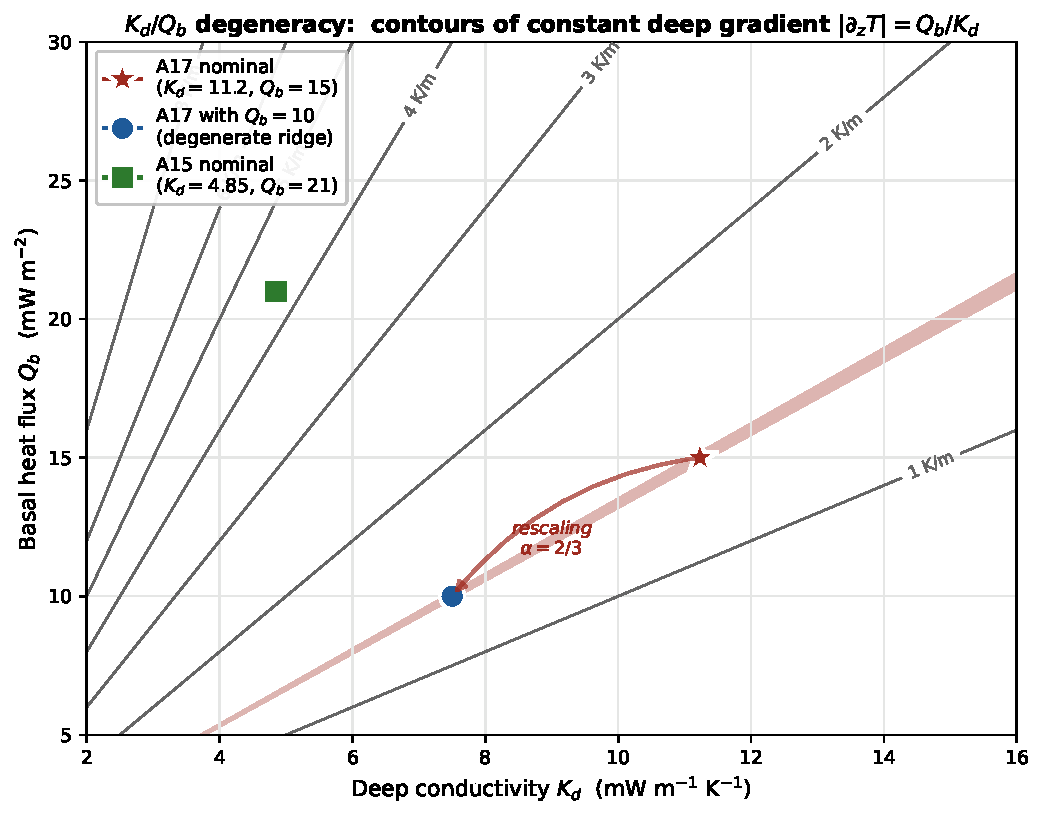
\includegraphics[width=0.78\linewidth]{figures/fig_kd_qb_degeneracy.pdf}
\caption{\textbf{The $K_d / Q_b$ degeneracy of single-borehole
inversions.} Grey contours show curves of constant deep equilibrium
gradient $|\partial_z T| = Q_b/K_d$. The Apollo~17 retrieval (red
star) and the Apollo~15 retrieval (green square) sit on different
contours, confirming that the inter-site contrast is not a $Q_b$
artefact. The blue circle shows where the A17 retrieval would move
if the basal heat flux were closer to the
\citet{saito2007,nagihara2018} reanalysis value of
$\sim\!10\,\si{\milli\watt\per\meter\squared}$: the rescaling
($\alpha=2/3$, red arrow) slides the retrieval along the same
iso-gradient ridge from $(K_d,Q_b)=(11.2, 15)$ to
$(K_d,Q_b)=(7.5, 10)$. Crucially, this rescaling does not change
the equilibrium temperature profile, and so it is invisible to a
single-borehole inversion.}
\label{fig:degeneracy}
\end{figure}

\section{Joint Bayesian posterior in $(K_d, Q_b)$}\label{sec:posterior}

We complement the profile-likelihood bootstrap of the main letter
with a proper Bayesian posterior on $(K_d, Q_b)$ at each Apollo
site. The likelihood is Gaussian in the deep-sensor profile
residual, $\mathcal{L}(K_d, Q_b) \propto \exp[-\tfrac{1}{2}\,
N_\mathrm{deep}\,\mathrm{RMSE}^2(K_d, Q_b)/\sigma_\mathrm{data}^2]$
with $\sigma_\mathrm{data}=\SI{0.5}{\kelvin}$. In the
conduction-dominated regime the deep equilibrium profile depends
on $(K_d, Q_b)$ only through their ratio, $|\partial_z T|=Q_b/K_d$;
we therefore evaluate the likelihood at any candidate $(K_d, Q_b)$
by interpolating the published-$Q_b$ RMSE-vs-$K_d$ curve at the
``effective'' conductivity $K_\mathrm{eff} = K_d\,(Q_b^\mathrm{pub}/Q_b)$,
which exactly preserves the degeneracy. A Gaussian prior on $Q_b$
captures the \citet{saito2007,nagihara2018} reanalysis envelope:
$Q_b\sim\mathcal{N}(\SI{18}{\milli\watt\per\meter\squared}, \SI{5}{\milli\watt\per\meter\squared})$ at A15 and
$Q_b\sim\mathcal{N}(\SI{13}{\milli\watt\per\meter\squared}, \SI{4}{\milli\watt\per\meter\squared})$ at A17. The prior on $K_d$ is flat in $\log K_d$
within $[10^{-3},\,30\times 10^{-3}]$\,\si{\watt\per\meter\per\kelvin}.

The posterior is sampled with the affine-invariant
ensemble sampler \texttt{emcee}
\citep{foreman_mackey2013emcee}: 32 walkers, 4000 steps, the first
1000 steps discarded as burn-in. Convergence is assessed by the
integrated autocorrelation length, which is $\sim 50$\,steps per
walker at both sites, giving $> 1000$ effectively-independent
samples per parameter. The marginal-posterior summary statistics
are
\[
\begin{array}{lcc}
\toprule
& \text{Apollo 15} & \text{Apollo 17} \\
\midrule
K_d \text{ (median, mW\,m$^{-1}$\,K$^{-1}$)} & 3.78 & 13.25 \\
K_d \text{ (16/84 percentiles)}              & 2.59,\,5.08 & 7.15,\,23.19 \\
K_d \text{ (95\% credible interval)}         & {[1.55,\,6.50]} & {[3.56,\,28.58]} \\
Q_b \text{ (median, mW\,m$^{-2}$)}            & 16.3 & 11.1 \\
\bottomrule
\end{array}
\]
The posterior on $K_d$ is wider than the bootstrap CI in the main
letter because it is propagating the full prior-driven $Q_b$
uncertainty along the iso-ratio ridge in addition to the
sensor-resampling uncertainty. The two summaries answer different
questions and should be reported alongside each other: the
bootstrap CI is the appropriate uncertainty when $Q_b$ is treated
as a fixed input, while the posterior is the appropriate
uncertainty when $Q_b$ is treated as Bayesian-uncertain. In both
treatments, the inter-site contrast remains robust because the
$K_d/Q_b$ degeneracy ridge constrains both sites identically.

\begin{figure}[hbt]
\centering
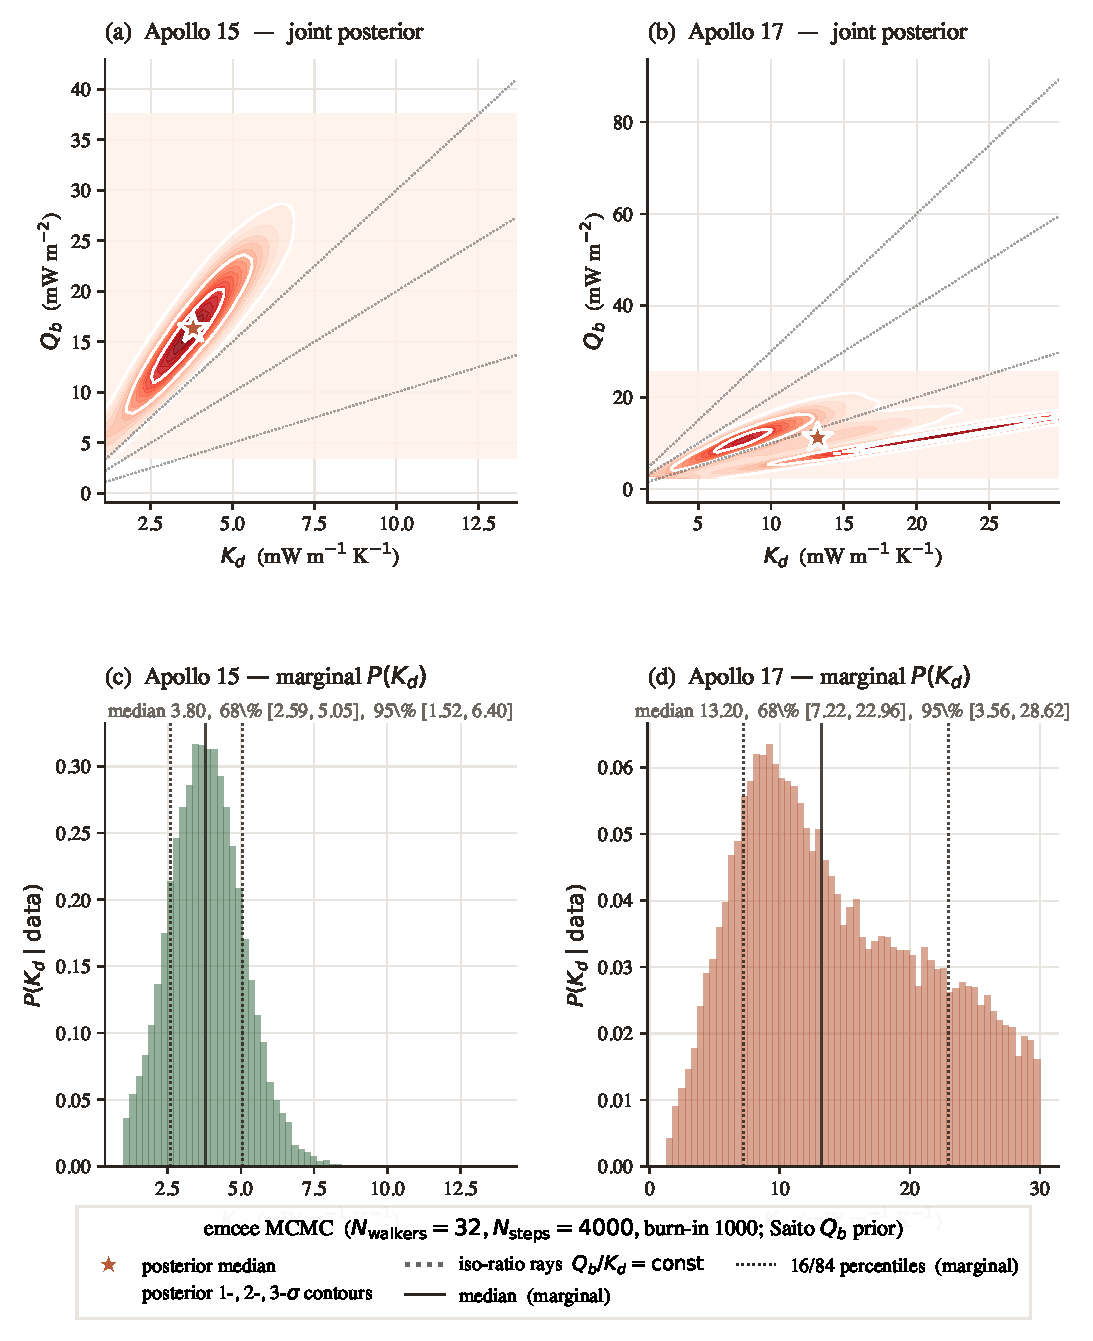
\includegraphics[width=\linewidth]{figures/fig_kd_qb_posterior.pdf}
\caption{\textbf{Bayesian posterior on $(K_d, Q_b)$ from
\texttt{emcee} MCMC at the two Apollo sites.} Panels (a)--(b):
joint posterior densities; the red star is the posterior median,
white contours enclose the inner 5\%, 32\%, and 68\% probability
regions, and the dotted grey lines are iso-ratio rays
$Q_b/K_d=\mathrm{const}$ along which the equilibrium temperature
profile is invariant. Panels (c)--(d): marginal posteriors on
$K_d$ (filled histograms) with median (solid) and 16/84
percentiles (dotted) annotated. The wider $K_d$ posterior at A17
reflects the long iso-ratio tail toward higher $K_d$ paired with
lower $Q_b$.}
\label{fig:posterior}
\end{figure}

% =====================================================================
\chapter{The Numerical Solver}\label{ch:numerics}

\section{Discretisation strategy}

The depth grid is geometrically expanding so that the surface skin
($\sim\!\delta_\mathrm{diurnal}\!\sim\!\SI{6}{\centi\meter}$) is
resolved at $\sim\!\SI{2}{\milli\meter}$ while the deep column
($\sim\!\SI{5}{\meter}$) is reached in $\sim\!120$ cells:
\[
z_0 = 0,\qquad
z_{i+1} - z_i = \Delta z_0 \cdot (1+g)^{\,i},\qquad
\Delta z_0 = \SI{2}{\milli\meter},\;\; g = 0.08.
\]
Time discretisation uses a fixed $\Delta t = 1\,\si{\hour}$, giving
$24\times29.53 = 708.7$ steps per lunation.

\section{Crank-Nicolson scheme}
Writing $T_i^n \equiv T(z_i, t_n)$ and discretising
(\ref{eq:heat-rep}) symmetrically in time gives a tridiagonal linear
system at each step:
\begin{equation}
T_i^{n+1} - T_i^n
   = \tfrac{1}{2}\,\frac{\Delta t}{\rho_i c_{p,i}}
     \Bigl[\mathcal{D}T^{n+1} + \mathcal{D}T^n\Bigr]_i,
\label{eq:CN}
\end{equation}
with $\mathcal{D}$ the 2nd-order finite-difference operator
\[
[\mathcal{D}T]_i = \frac{1}{\Delta z_i}\!\left[
   \frac{K_{i+\tfrac12}}{\Delta z_{i+\tfrac12}}\bigl(T_{i+1}-T_i\bigr)
   - \frac{K_{i-\tfrac12}}{\Delta z_{i-\tfrac12}}\bigl(T_i-T_{i-1}\bigr)
\right]
\]
on the interior, and modified rows for the radiative-BC top
(\ref{eq:bc-top-rep}, requiring an outer Picard iteration to handle
$T_s^4$) and the imposed-flux bottom (\ref{eq:bc-bot-rep}).
The system is solved with the Thomas algorithm
\citep[$O(N_z)$;][]{press2007}.

\begin{aside}[Why Crank-Nicolson and not pure-implicit Euler?]
Pure-implicit Euler is unconditionally stable but only first-order
accurate in time, which damps the diurnal wave artificially and
produces a $\sim\!\SI{2}{\kelvin}$ amplitude error at the top sensors
even at $\Delta t = \SI{1}{\hour}$. Crank-Nicolson is also
unconditionally stable but second-order accurate, eliminating the
spurious damping. The cost is a slightly more complex tridiagonal
right-hand side, paid once per step.
\end{aside}

\section{Spin-up}
The initial condition $T(z,t=0) = T_\mathrm{init}$ (a constant
matching each site's annual-mean Diviner brightness, irrelevant after
spin-up) is propagated for 100 lunations. We declare convergence
when $\max_i|T_i^{n+L} - T_i^n| < 10^{-2}\,\si{\kelvin}$ over a full
lunation $L$. Fig.~\ref{fig:spinup} confirms that 100 lunations
reach $\sim\!10^{-3}\,\si{\kelvin}$ everywhere, well below the
declared tolerance.

\begin{figure}[t]
\centering

\includegraphics[width=0.85\linewidth]{figures/apollo_spinup_convergence.pdf}
\caption[Spin-up convergence diagnostic]{\textbf{SI Fig.~S6 ---
Spin-up convergence diagnostic.} Maximum per-lunation
$\Delta T = \max_i|T_i^{n+L} - T_i^n|$ as a function of lunation
number, for the \Hayne\ reference model at both Apollo sites. The
dashed line is the $10^{-2}\,\si{\kelvin}$ convergence threshold;
both sites comfortably pass at 100 lunations.}
\label{fig:spinup}
\end{figure}

% =====================================================================
\chapter{Apollo HFE Validation in Detail}\label{ch:validation}

This chapter documents the four supplementary diagnostic figures that
underpin the validation claims of the main Letter. The figures are
generated by the companion notebook
\texttt{01b\_apollo\_SI.ipynb} (Figs.~S1--S6) and by the main notebook
\texttt{01\_apollo\_validation.ipynb} (Figs.~S7--S11).

\section{Per-sensor diurnal grid}\label{sec:per-sensor}

Letter Fig.~3 shows the diurnal cycle at the deepest TG sensor only,
to keep the headline figure uncluttered. The complete per-sensor
grids for both Apollo sites are reproduced as Figs.~\ref{fig:S1} and
\ref{fig:S2} below, including the shallow ($z<\zborestem$) sensors
that are excluded from the quantitative RMSE. The shaded red panels
highlight the borestem-contaminated zone and let the reader see at a
glance that the model \emph{should not} reproduce those sensors.

\begin{figure}[p]
\centering

\includegraphics[width=0.92\linewidth]{figures/a15_diurnal_sensor_grid.pdf}
\caption[A15 diurnal grid]{\textbf{SI Fig.~S1 --- Apollo~15 per-sensor
phase-folded diurnal cycle.} Each panel shows one HFE sensor
(deep~$=$~green border, shallow/borestem~$=$~red border). Black
markers are the SPICE-LST-folded median of the observed temperature;
coloured lines are the \Hayne\ (navy) and Discrete (grey) modelled
diurnal swing at the same depth, peak-aligned to the observed
maximum (faint ghost lines $=$ unshifted model).}
\label{fig:S1}
\end{figure}

\begin{figure}[p]
\centering

\includegraphics[width=0.92\linewidth]{figures/a17_diurnal_sensor_grid.pdf}
\caption[A17 diurnal grid]{\textbf{SI Fig.~S2 --- Apollo~17 per-sensor
phase-folded diurnal cycle.} Conventions as in Fig.~\ref{fig:S1}.}
\label{fig:S2}
\end{figure}

\section{One-to-one obs vs model scatter}
Fig.~\ref{fig:S3} collapses every sensor at both sites onto a
single 1:1 plot. The deep sensors (filled markers) lie close to the
diagonal at both sites, while the shallow sensors (open markers)
scatter systematically off it --- the warm side, as expected from
the borestem heat-short.

\begin{figure}[t]
\centering

\includegraphics[width=0.78\linewidth]{figures/apollo_obs_vs_model_scatter.pdf}
\caption[Obs vs model scatter]{\textbf{SI Fig.~S3 --- Observed vs
modelled equilibrium temperature, both sites and both models.}
Filled markers $=$ deep sensors ($z>\zborestem$); open markers $=$
shallow sensors. The dashed line is the 1:1 reference.}
\label{fig:S3}
\end{figure}

\section{Residual vs depth}
Fig.~\ref{fig:S4} plots the per-sensor residual ($T_\mathrm{model}
- T_\mathrm{obs}$) against depth. Two features should be noted:
(i)~the deep ($z>\zborestem$) residuals are zero-mean within
$\sim\!1\,\si{\kelvin}$ for both models at A15, and zero-mean
for the Discrete model at A17 while the Hayne model has a
$+\SI{2.5}{\kelvin}$ deep bias; (ii)~the shallow residuals trend
monotonically negative (model too cold) above $\zborestem$, the
expected signature of a heat source not in the model --- i.e.\ the
borestem.

\begin{figure}[t]
\centering

\includegraphics[width=0.78\linewidth]{figures/apollo_residual_vs_depth.pdf}
\caption[Residual vs depth]{\textbf{SI Fig.~S4 --- Per-sensor
residual ($T_\mathrm{model} - T_\mathrm{obs}$) versus sensor depth,
both sites and both models.} The lavender band marks the borestem
exclusion zone.}
\label{fig:S4}
\end{figure}

\section{Diurnal amplitude vs depth (the borestem signature)}\label{sec:borestem-diag}
This is the diagnostic figure that motivates our \emph{a priori}
exclusion of $z<\zborestem$. The modelled diurnal amplitude
attenuates exponentially with depth at the rate predicted by
(\ref{eq:skin}); the observed amplitude follows the same exponential
\emph{below} $\zborestem$ but \emph{flares} sharply above it,
indicating an additional heat source --- the borestem --- that the
regolith model does not include.

\begin{figure}[t]
\centering

\includegraphics[width=0.78\linewidth]{figures/apollo_amplitude_vs_depth.pdf}
\caption[Amplitude vs depth]{\textbf{SI Fig.~S5 --- Diurnal amplitude
versus sensor depth, observed (black) vs modelled (Hayne, navy).}
The model attenuates as predicted by (\ref{eq:skin}); the observations
flare sharply above $\zborestem$, the borestem signature.}
\label{fig:S5}
\end{figure}

\begin{aside}[Mild deep-amplitude under-prediction at A17]
A close inspection of Fig.~\ref{fig:S5} shows that, below
$\zborestem$ at the A17 borehole, the observed diurnal
amplitudes sit slightly above the \Hayne\ model envelope (by
$\sim\!0.05$--$0.10\,\si{\kelvin}$, comparable to the digitisation
noise floor of the restored 1975--1977 records used here).
The 3-layer discrete model reduces this gap by raising
$K_d^\mathrm{disc}$ to $6.3\times10^{-3}$, which lengthens the
diurnal skin depth and lifts the deep-sensor amplitude envelope.
This is the same mechanism that drives the A17 RMSE improvement
in Letter Table~1, and it points to the deep conductivity --- not
the shallow profile --- as the parameter most worth refining
against in-situ data. A dense $K_d$ sweep is deferred to the
Phase-2 regression companion, where it can be carried out jointly
with $Q_b$ retrieval to break the well-known $K_d/Q_b$ degeneracy.
\end{aside}

% =====================================================================
\chapter{Independent Cross-Checks}\label{ch:crosschecks}

\section{Surface temperature against Diviner}
The radiative top boundary condition (\ref{eq:bc-top-rep}) implicitly
predicts the lunar surface skin temperature
$T_s(t)\equiv T(0,t)$. We compare the modelled
$T_s^\mathrm{max}/T_s^\mathrm{min}$ at each site to the
Diviner-measured lat-band envelope reported by \Vas\ (their Fig.~7)
and find agreement to within the Diviner uncertainty
(Fig.~\ref{fig:S7}).

\begin{figure}[t]
\centering

\includegraphics[width=0.85\linewidth]{figures/phase1_surface_T_diviner_check.pdf}
\caption[Surface T vs Diviner]{\textbf{SI Fig.~S7 --- Modelled
surface skin temperature vs.\ Vasavada et~al.\ (2012)
Diviner mean lat-band envelope at the Apollo 15 and 17 latitudes.}
Bars are the modelled ($T_s^\mathrm{min}$, $T_s^\mathrm{max}$);
dashed lines are the Vasavada Fig.~7 lat-band typical maxima.}
\label{fig:S7}
\end{figure}

\section{Topographic shadow algorithm}
Phase~1 of the pipeline assumes a flat horizon at both Apollo
sites; the assumption must be \emph{verified}, not asserted, because
the same DEM/horizon machinery will be applied to the rugged polar
sites in Phase~2.

\subsection{Flat-plain horizon \emph{unit test} (S8)}
Fig.~\ref{fig:S8} is a \textbf{unit test of the horizon ray-marcher},
not a scientific result. It exercises the
\citet{mazarico2011}-style ray-march algorithm on a synthetic
flat-plain DEM (constant elevation everywhere) and confirms that
the recovered horizon angle is below $0.05^\circ$ in all azimuths,
i.e.\ the algorithm correctly returns ``no horizon'' on input that
has none. This is a standard regression check on the Phase-2
horizon code path, which we exercise here so that the same
implementation can be deployed without modification to the
\textbf{rugged polar sites} of Phase~2 (where the horizon is far
from flat and dominates the local energy balance).
The companion crater unit test (Fig.~\ref{fig:S9}) confirms that
the same code recovers the correct non-trivial horizon profile
when fed a non-flat DEM.

\begin{aside}[Phase-2 LOLA test plan]
For Phase~2 the same ray-marcher will be driven by LOLA
$\sim\!\SI{20}{\meter}$/pixel polar DEMs at PSR-rim candidate
sites; the unit-test pair S8/S9 is the regression suite that the
implementation is locked against. The Phase-2 paper will report
the science output of the horizon-aware solver at those rugged
sites; here we publish only the test fixtures.
\end{aside}

\begin{figure}[t]
\centering

\includegraphics[width=0.78\linewidth]{figures/apollo_flat_horizon_check.pdf}
\caption[Flat horizon unit test]{\textbf{SI Fig.~S8 --- Unit test of
the horizon ray-marcher on a synthetic flat-plain DEM at the
Apollo~15 and~17 latitudes.} Maximum recovered horizon elevation
angle vs.\ azimuth, extracted with the \citet{mazarico2011}-style
ray-march. Recovered angle $<0.05^\circ$ everywhere confirms the
algorithm returns ``no horizon'' on input that has none. This is a
regression check on the Phase-2 polar code path, not a scientific
result for Apollo --- the flat-horizon assumption at Apollo is
already justified by site selection (mare).}
\label{fig:S8}
\end{figure}

\subsection{Crater horizon regression (S9)}
The same horizon tracer is exercised on a synthetic crater
(diameter \SI{1}{\kilo\meter}, depth \SI{200}{\meter}) to confirm
that it correctly recovers a non-trivial horizon profile
(Fig.~\ref{fig:S9}).

\begin{figure}[t]
\centering

\includegraphics[width=0.78\linewidth]{figures/phase1_crater_horizon_check.pdf}
\caption[Crater horizon test]{\textbf{SI Fig.~S9 ---
\citet{mazarico2011} horizon tracer regression test on a synthetic
crater DEM (diameter \SI{1}{\kilo\meter}, depth \SI{200}{\meter}).
Recovered horizon (markers) vs.\ analytic crater rim profile
(dashed).}}
\label{fig:S9}
\end{figure}

\subsection{Insolation chain demo (S10)}
Fig.~\ref{fig:S10} shows the end-to-end DEM~$\rightarrow$~horizon
mask~$\rightarrow$~insolation chain on the same crater DEM, with
the shadow boundary correctly tracked across a full diurnal cycle.

\begin{figure}[t]
\centering

\includegraphics[width=0.85\linewidth]{figures/phase1_insolation_shadow_demo.pdf}
\caption[Shadow demo]{\textbf{SI Fig.~S10 --- DEM
$\rightarrow$ horizon mask $\rightarrow$ instantaneous insolation,
illustrated on the synthetic crater of Fig.~\ref{fig:S9} at three
solar times.}}
\label{fig:S10}
\end{figure}

\subsection{Shadow-coupled solver closure (S11)}
The most stringent check: hooking the shadow mask into the actual
1-D solver and confirming that, on a flat plain (where the mask is
identically~1), the solver reproduces the no-shadow baseline to
better than \SI{0.05}{\kelvin} everywhere
(Fig.~\ref{fig:S11}).

\begin{figure}[t]
\centering

\includegraphics[width=0.78\linewidth]{figures/phase1_shadow_solver_closure.pdf}
\caption[Solver closure]{\textbf{SI Fig.~S11 --- Shadow-coupled
1-D solver closure test.} Difference between the shadow-coupled and
no-shadow solver output on a flat-plain DEM. Maximum
$|\Delta T|<\SI{0.05}{\kelvin}$ everywhere confirms that the shadow
hook is correctly disabled when the mask is unity.}
\label{fig:S11}
\end{figure}

% =====================================================================
\chapter{Reproducibility \& Code Walk-through}\label{ch:repro}

The complete Phase-1 pipeline is open-source and lives at
\url{https://github.com/rp3gregorio/Lunar-V2}, branch
\texttt{claude/cleanup-repo-organization-EcS3U}. Two notebooks
reproduce every figure in this document:

\begin{itemize}\itemsep2pt
  \item \texttt{notebooks/phase1\_validation/01\_apollo\_validation.ipynb}
        --- main notebook: reproduces Letter Figs.~1--4, Table~1,
        and SI Figs.~S7--S11.
  \item \texttt{notebooks/phase1\_validation/01b\_apollo\_SI.ipynb}
        --- companion: reproduces SI Figs.~S1--S6.
\end{itemize}

\section{Repository layout (Phase 1)}
\begin{lstlisting}[language=bash,caption={Top-level layout of the
Phase-1 deliverables.}]
Lunar-V2/
  lunar/
    constants.py        # Physical constants + Hayne 2017 fit values
    properties.py       # K(T,z), rho(z), c_p(T) implementations
    solver.py           # Crank-Nicolson 1-D solver + boundary BCs
    illumination.py     # DEM, horizon tracer, shadow mask
    apollo_helpers.py   # Per-site solver dispatch + stats
    plotting/
      style_guide.py    # GRL-style mpl rcParams + colour palette
  notebooks/phase1_validation/
    01_apollo_validation.ipynb   # Main letter notebook
    01b_apollo_SI.ipynb          # SI companion notebook
  data/
    apollo/             # HFE restored record (Nagihara+2018)
    spice/              # JPL SPICE kernels (DE440, MOON_ME)
\end{lstlisting}

\section{Minimal solver invocation}
The following $\sim\!30$ lines reproduce the \Hayne\ Apollo 15 result
of Table~1:
\begin{lstlisting}[caption={Minimal Apollo 15 \Hayne\ run.},
                   label={lst:minimal}]
import numpy as np
from lunar.constants  import (S0, K_SURFACE, K_DEEP, H_PARAMETER,
                              CHI_RADIATIVE, T_REFERENCE,
                              RHO_SURFACE, RHO_DEEP)
from lunar.properties import (conductivity_hayne, density_hayne,
                              specific_heat)
from lunar.solver     import PixelInputs, run_pixel
from lunar.apollo_helpers import build_insolation_for_site, A15_SITE

# 1. Build the surface forcing F_solar(t) at Apollo 15 via SPICE.
t_sec, insolation = build_insolation_for_site(A15_SITE,
                                              n_lunations=100)

# 2. Wire the Hayne 2017 property functions into the solver.
inp = PixelInputs(
    t = t_sec,
    z_max = 5.0, dz0 = 2e-3, growth = 0.08,
    K_func   = lambda T, z: conductivity_hayne(T, z,
                K_SURFACE, K_DEEP, H_PARAMETER, CHI_RADIATIVE),
    rho_func = lambda z:    density_hayne(z, RHO_SURFACE,
                                          RHO_DEEP, H_PARAMETER),
    cp_func  = lambda T:    specific_heat(T, model='hayne'),
    insolation = insolation,
    albedo = A15_SITE['albedo'],
    emissivity = A15_SITE['emissivity'],
    Q_b = A15_SITE['Q_BASAL'],
    T_init = 250.0,
    spinup_lunations = 100, spinup_tol_K = 1e-2,
)

# 3. Solve and inspect.
out = run_pixel(inp)
print(f"Deep T(z=1m)  = {np.interp(1.0, out.z, out.T.mean(axis=1)):.2f} K")
print(f"Surface T_max = {out.T_surface.max():.1f} K")
\end{lstlisting}

\section{How to swap the regolith model}
Because \texttt{PixelInputs} accepts the property functions
($K$, $\rho$, $c_p$) as kwargs, swapping to the Discrete-3-layer or
to the Biele-2022 $c_p$ rational fit is a two-line change:
\begin{lstlisting}[caption={Discrete 3-layer + Biele $c_p$ swap.}]
from lunar.properties import conductivity_discrete

inp = inp._replace(
    K_func  = lambda T, z: conductivity_discrete(T, z),
    cp_func = lambda T:    specific_heat(T, model='biele'),
)
out_alt = run_pixel(inp)
\end{lstlisting}
The full sensitivity sweep of Letter Fig.~4 is implemented as a loop
over these two-line swaps, which is why the cell is short and easy
to audit.

% =====================================================================
\chapter{Supplementary letter figures}\label{ch:letter-figs}

This chapter collects four auxiliary figures that were promoted from
the main letter to the SI in order to keep the letter within
JGR:Planets length conventions. The references in the main letter
text point to the labels defined here.

\section{Provenance check of the regolith property functions}

\begin{figure}[htbp]
\centering

\includegraphics[width=0.92\linewidth]{figures/fig1_hayne_model_properties.pdf}
\caption{\textbf{Provenance check of the regolith property functions
implemented in the solver.} (a)~Thermal conductivity
$K(T{=}\SI{250}{\kelvin},z)$: the \Hayne\ smooth H-parameter form
and the \citet{martinez2021}-style 3-layer alternative
super-imposed; both include the same radiative multiplier
$1+\chi(T/T_\mathrm{ref})^3$. (b)~Surface $K(T,z\!\to\!0)$ vs.\ $T$.
(c)~Bulk density $\rho(z)$ and the 3-layer continuation toward
$\rho_\mathrm{max}$. (d)~Specific heat $c_p(T)$ from the
Hemingway--Robie--Wilson polynomial reproduced in the
\Hayne\ Appendix. The four parameterised inputs match the published
\Hayne\ figures.}
\label{fig:hayne-props-SI}
\end{figure}

\section{Auxiliary parameter sensitivity}

\begin{figure}[htbp]
\centering

\includegraphics[width=\linewidth]{figures/fig4_sensitivity_suite.pdf}
\caption{\textbf{Parameter-sensitivity suite for the \Hayne\
reference model.} Deep-sensor RMSE versus (a) basal heat flux
$Q_b$, (b) radiative-conductivity coefficient $\chi$ (\Hayne\
default $\chi=2.7$ marked), and (c) specific-heat parameterisation.
Shaded ranges span the published uncertainty of each parameter; the
deep RMSE shifts by $<\SI{0.5}{\kelvin}$ across all sweeps. $K_d$
is treated separately as the controlled retrieval parameter in the
main letter.}
\label{fig:sensitivity-SI}
\end{figure}

\section{Comparison of $K_d$ across measurement scales}

\begin{figure}[htbp]
\centering
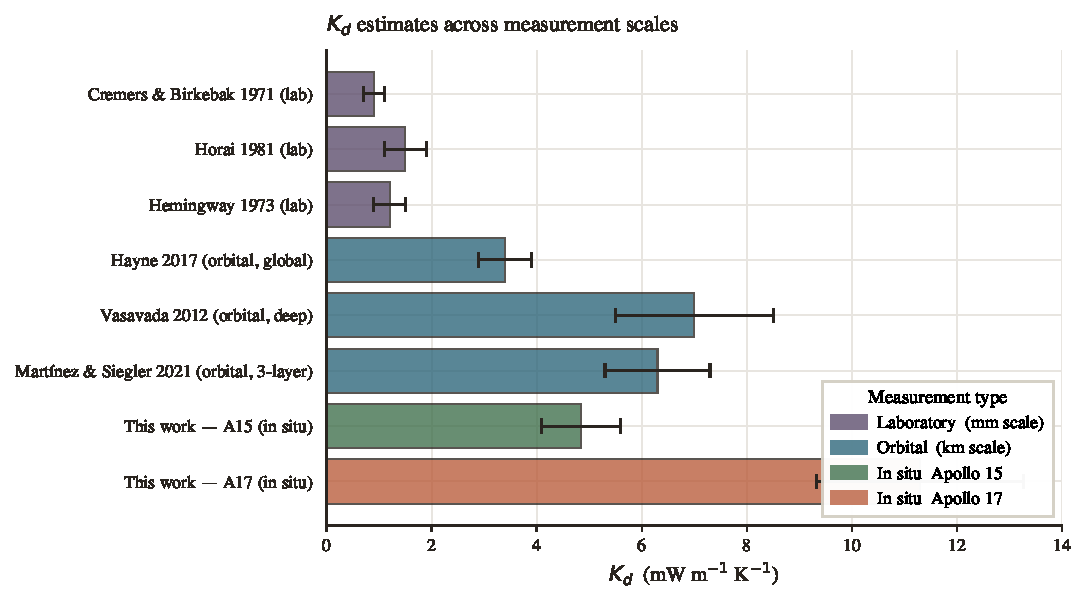
\includegraphics[width=0.92\linewidth]{figures/fig_lab_comparison.pdf}
\caption{\textbf{$K_d$ estimates across measurement scales.}
Laboratory measurements on returned Apollo regolith samples
\citep{cremers1971,horai1981,hemingway1973} cluster at
$\sim\!1\,\si{\milli\watt\per\meter\per\kelvin}$; orbital fits
\citep{hayne2017,vasavada2012,martinez2021} span
$\sim\!3$--$\SI{7e-3}{\watt\per\meter\per\kelvin}$; the present
in-situ retrievals lie at $\sim\!5$ (A15) and $\sim\!11$ (A17)
mW\,m$^{-1}$\,K$^{-1}$.}
\label{fig:lab-comparison-SI}
\end{figure}

\section{Implication for polar-volatile cold-trap depth}

\begin{figure}[htbp]
\centering
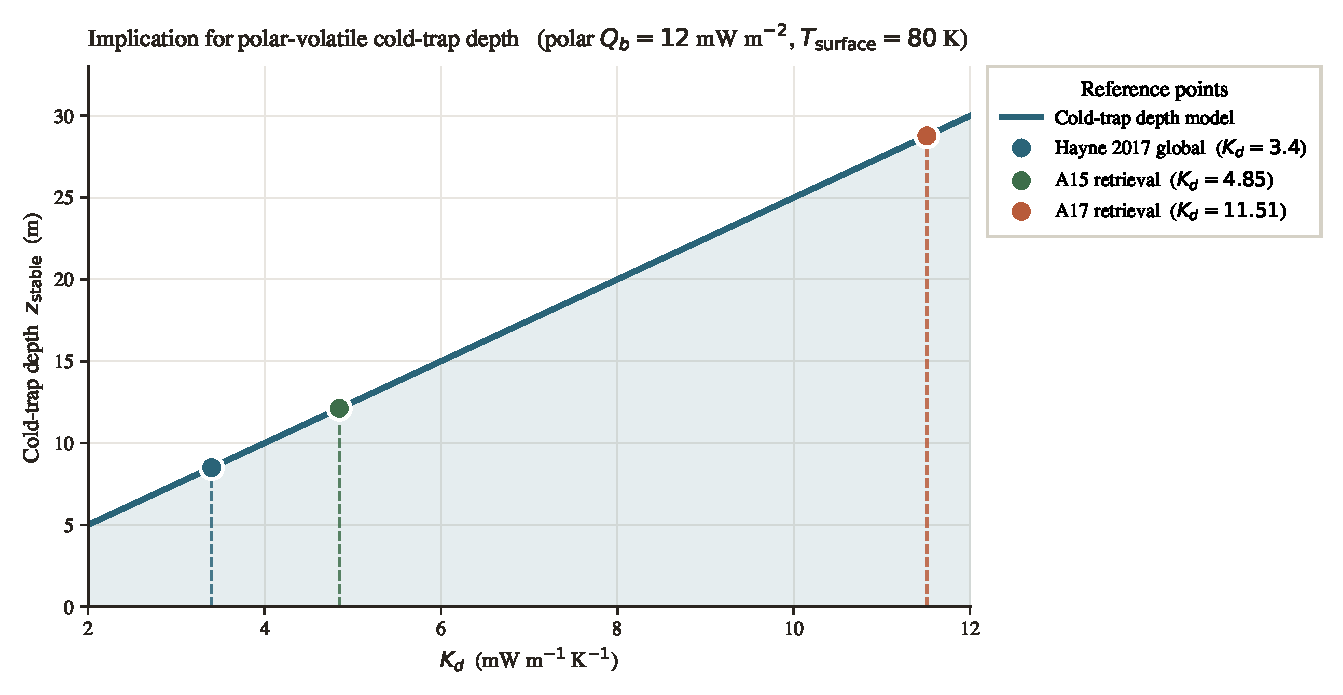
\includegraphics[width=0.78\linewidth]{figures/fig_cold_trap_depth.pdf}
\caption{\textbf{Implication for polar volatile cold-trap depth.}
Indicative cold-trap depth $z_\mathrm{stable}$ at which buried
water ice is thermally stable on geological timescales (a
\citealt{schorghofer2005}-style estimate at fixed polar surface
temperature and basal heat flux), as a function of $K_d$. The
factor-of-$\sim\!3$ change in $K_d$ between the global value of
\citet{hayne2017} and the A17 retrieval translates into a
factor-of-$\sim\!3$ change in $z_\mathrm{stable}$, illustrating
that the regional heterogeneity in $K_d$ reported here is large
enough to matter for downstream volatile-stability budgets.}
\label{fig:cold-trap-SI}
\end{figure}

\section{Surface-temperature closure against Diviner}\label{sec:diviner-closure}

The deep $K_d$ retrieval reported in the main letter rests on the
assumption that the surface-forcing chain (SPICE/DE440 ephemerides,
Bond albedo, broadband emissivity) drives the model column with
realistic surface boundary conditions. Fig.~\ref{fig:diviner-SI}
provides an independent test: at each Apollo site the model surface
temperature trace (run with the per-site retrieved
$K_d^{*}$) is compared against the Diviner Lunar Radiometer Global
Cumulative Product \citep[GCP;][]{williams2017diviner} pixels at the
same latitude and within $\pm 1^\circ$ of the site longitude.

The model reproduces the Diviner diurnal shape --- terminator
timing, plateau width, and night-time floor --- to high fidelity at
both sites. The full-cycle RMSE between model and Diviner brightness
temperature is $12.5$\,K at A15 and $17.5$\,K at A17, with a model
warm-bias of $+5.0$ and $+9.1$\,K respectively
(Fig.~\ref{fig:diviner-SI}, panels a--b). The day-side component of
the residual is consistent with the well-documented anisothermal
footprint effect \citep{bandfield2015,hayne2017}: the GCP grid pixel
mixes sub-pixel-scale shadows, slopes, and rocks, which broaden the
distribution of effective temperatures and reduce the peak
brightness compared to a 1-D homogeneous radiative-equilibrium
model.

The night-side residual (Fig.~\ref{fig:diviner-SI}, panels c--d)
is dominated by a different mechanism. Restricting the residual to
local solar time $<\!6$ or $\geq\!18$ gives RMSE values of $12.0$
and $21.8$\,K at A15 and A17 respectively, with biases of $+10.2$
and $+21.6$\,K. Because the anisothermal effect is largest in the
day (when sub-pixel illumination differences are large) and small
at night, the persistent night-side warm bias is most likely a
forcing-side parameter offset --- in particular, the bolometric
albedo and broadband emissivity adopted from
\citet{vasavada2012,bandfield2015} are latitude-band averages
rather than measured values at the A15 / A17 footprints. Local
albedo or emissivity differing by 1--2\% from the lat-band mean
would account for a $\sim$10\,K shift in the night-side temperature.

Crucially, neither residual propagates into the deep $K_d$
retrieval. The deep equilibrium temperature is $T_d = T_\mathrm{surface}^{(\mathrm{mean})} + Q_b\!\int_0^{z_d}\!dz'/K(z')$;
a uniform shift in the surface mean (the only kind of offset
indicated by the night-side bias) shifts the absolute deep $T$ but
not the deep \emph{gradient}, which is what the $K_d$ retrieval
fits. The Diviner closure therefore confirms diurnal-shape fidelity
without contaminating the central retrieval.

\begin{figure}[hbt]
\centering
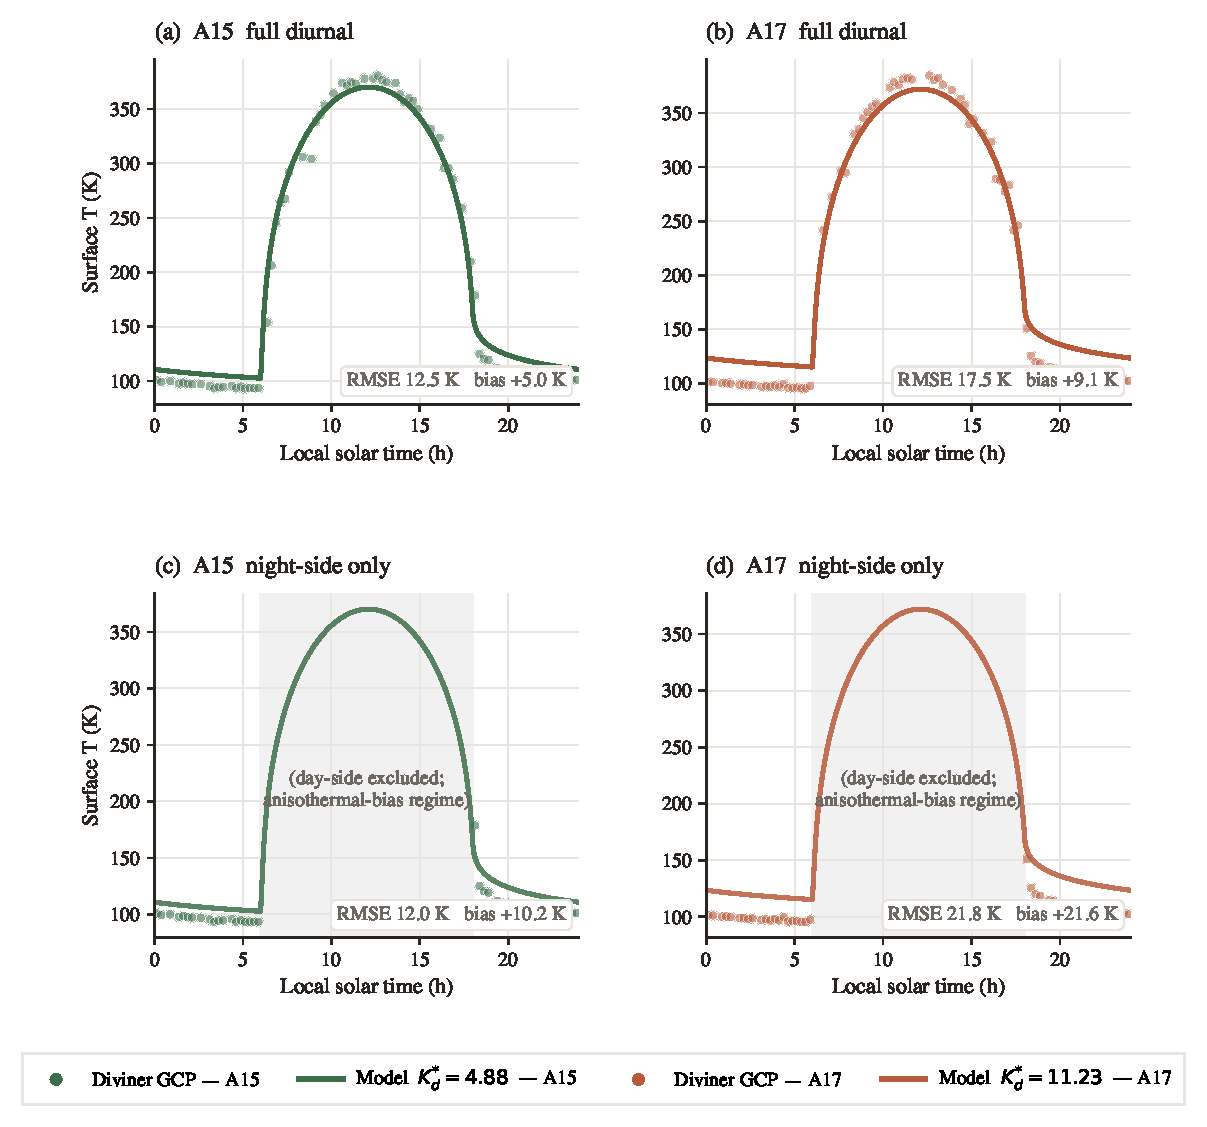
\includegraphics[width=\linewidth]{figures/fig_diviner_closure.pdf}
\caption{\textbf{Surface-temperature closure against the Diviner
GCP.} (a)--(b) Full diurnal cycle at each site: dots are the
Diviner brightness temperature binned at $0.25$-h LST resolution
within $\pm 0.5^\circ$ latitude and $\pm 1^\circ$ longitude of
each landing site; solid curves are the modelled surface
temperature run with the per-site retrieved $K_d^{*}$.
(c)--(d) Night-side-only restriction (LST in $[0,\,6)\cup[18,\,24]$;
day-side shaded). The full-cycle bias has a daytime anisothermal
component plus a residual night-side offset that is most plausibly
caused by local-scale bolometric-albedo / emissivity variations.
Neither component propagates into the deep $K_d$ retrieval, which
constrains the deep equilibrium gradient $Q_b/K_d$ and not the
absolute surface temperature.}
\label{fig:diviner-SI}
\end{figure}

\section{Held-out validation diagnostics}\label{sec:holdout}

The single-parameter $K_d$ retrieval reported in the main letter is
supported by two held-out diagnostics
(Fig.~\ref{fig:holdout-SI}). \emph{Panel (a)} reports the
TG\,vs.\,TR cross-prediction: at each site we fit $K_d$ using only
the gradient-bridge (TG) sensors and evaluate the deep RMSE on the
withheld ring-bridge (TR) sensors, and \emph{vice versa}. The
out-of-sample RMSEs match their in-sample counterparts to within
$\sim\!0.2$\,K, indicating that the two sensor populations are
mutually consistent under the same $K_d$ retrieval. \emph{Panel
(b)} reports a leave-one-out test in which the deepest sensor at
each site ($z = \SI{139}{\centi\meter}$ at A15,
$z = \SI{234}{\centi\meter}$ at A17) is withheld from the fit and
predicted by the remaining sensors. The model recovers the
withheld temperature to within
$|\Delta|=\SI{0.11}{\kelvin}$ (A15) and
$\SI{0.16}{\kelvin}$ (A17). Both diagnostics show that the
retrieval has out-of-sample skill, not just in-sample
goodness-of-fit.

\begin{figure}[hbt]
\centering
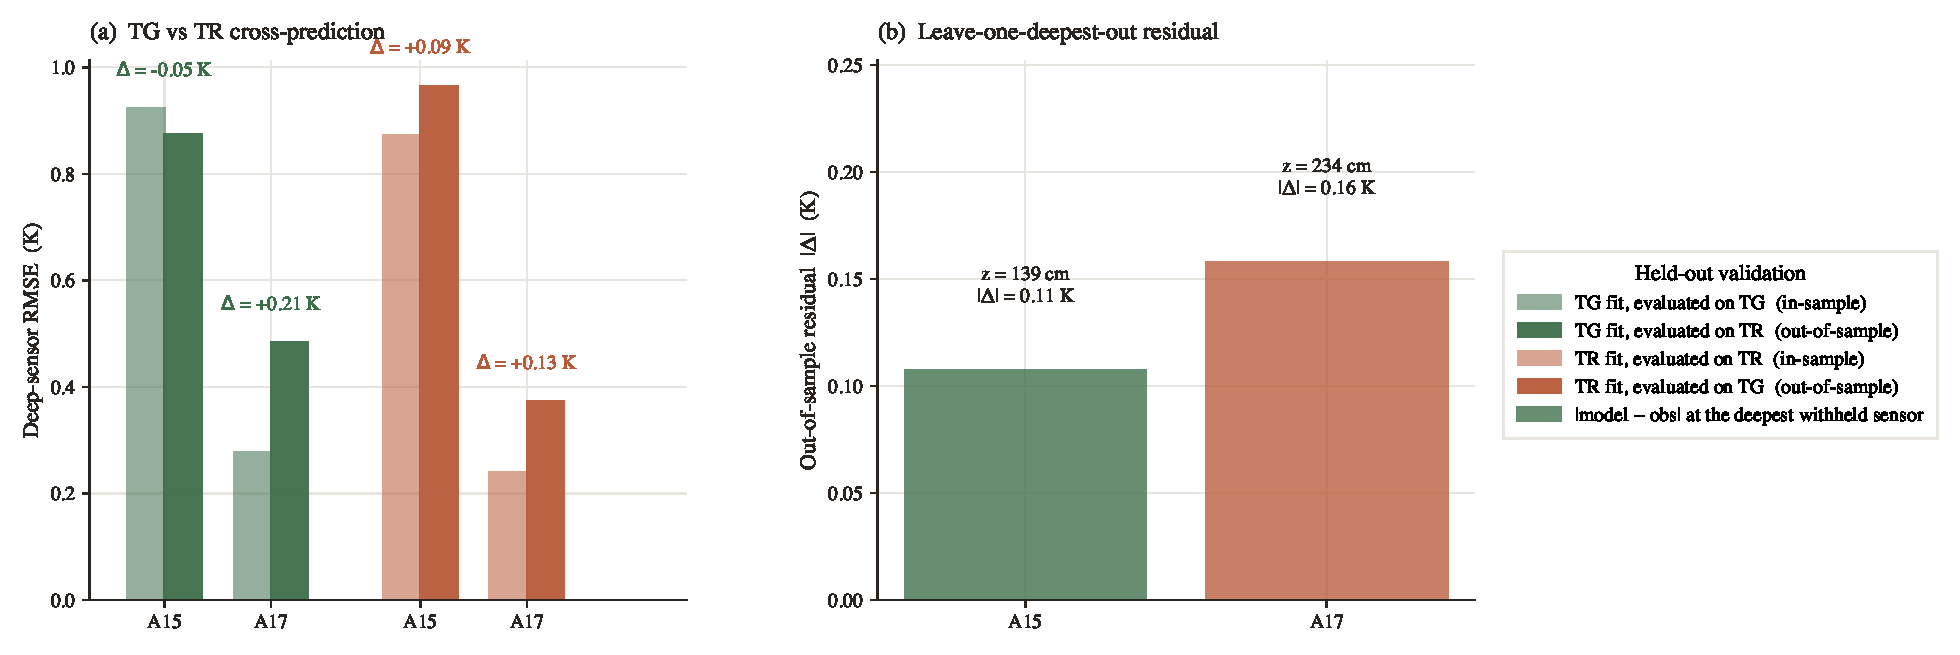
\includegraphics[width=\linewidth]{figures/fig_holdout.pdf}
\caption{\textbf{Held-out validation of the per-site $K_d$
retrieval.} (a)~TG\,vs.\,TR cross-prediction: open bars show the
in-sample deep RMSE achieved by the $K_d^{*}$ retrieval that uses
only the labelled sensor type; hatched bars show the
out-of-sample RMSE on the withheld sensor type. The
$\Delta$ annotations are the change between in-sample and
out-of-sample RMSE. (b)~Leave-one-out test on the deepest sensor
at each site: the bar height is the absolute residual at the
withheld sensor; the deepest-sensor depth is annotated.}
\label{fig:holdout-SI}
\end{figure}

% =====================================================================
\chapter{Glossary}\label{ch:glossary}

\begin{description}\itemsep2pt
  \item[ALSEP] \emph{Apollo Lunar Surface Experiments Package} ---
        the surface-mounted electronics box that powered and recorded
        each Apollo geophysical experiment, including the HFE.
  \item[Bond albedo $A$] The fraction of incident solar irradiance
        that a surface element scatters back to space integrated over
        all reflection angles and over the solar spectrum. For lunar
        regolith $A\!\sim\!0.07\text{--}0.14$ depending on terrain type.
  \item[Borestem] The fibreglass tube left in the HFE drill holes to
        keep them open. Source of the heat-short artefact discussed
        throughout this document.
  \item[Crank-Nicolson] An unconditionally stable, second-order-accurate
        time-discretisation scheme for parabolic PDEs (\citealt{press2007},
        Chap.~20).
  \item[DE440] JPL's current planetary ephemeris, providing positions of
        the Sun, Moon and planets accurate to $\sim\!\SI{2}{\meter}$ over
        modern times.
  \item[Diviner] The Diviner Lunar Radiometer Experiment on the Lunar
        Reconnaissance Orbiter \citep{paige2010} --- 9 broad-band channels
        between $0.3$ and \SI{400}{\micro\meter} measuring lunar
        brightness temperatures.
  \item[H-parameter ($H$)] The exponential length-scale of the depth
        dependence of $K(z)$ and $\rho(z)$ in the \Hayne\ model;
        $H=\SI{0.06}{\meter}$.
  \item[HFE] \emph{Heat-Flow Experiment}, the Apollo~15 and~17
        instrument that drilled boreholes and lowered platinum-resistance
        thermometers to measure the lunar geothermal heat flux.
  \item[LST] \emph{Local solar time}, the angular position of the Sun
        in the local sky, measured in lunar hours from local noon.
  \item[MOON\_ME] The body-fixed mean Earth/principal-axis frame for
        the Moon used by the SPICE toolkit; the standard reference
        frame for lunar-surface coordinates.
  \item[Skin depth $\delta$] The depth at which a periodic surface
        temperature wave attenuates by $e^{-1}$, defined in
        (\ref{eq:skin}). For the lunar diurnal wave,
        $\delta\sim\SI{6}{\centi\meter}$.
  \item[SPICE] NAIF's planetary geometry and ephemeris toolkit
        \citep{acton1996,acton2018}; the mission-grade source for $\theta_\odot$.
  \item[TG bridge] HFE \emph{thermal gradient} bridge: measures the
        temperature \emph{difference} between two sensors $\sim\!\SI{50}{\centi\meter}$
        apart along the borestem.
  \item[TR bridge] HFE \emph{thermometer ring} bridge: measures the
        \emph{absolute} temperature of a single sensor against a
        reference resistor in the ALSEP electronics.
  \item[Thermal inertia $I$] $\sqrt{K\rho c_p}$, defined in
        (\ref{eq:inertia}); the proportionality between surface
        temperature swing and inverse square-root of forcing frequency.
\end{description}

% =====================================================================
\bibliography{references}

\end{document}
